% Very simple template for lab reports. Most common packages are already included.
\documentclass[a4paper, 11pt]{article}
\usepackage[utf8]{inputenc} % Change according your file encoding
\usepackage{graphicx}
\usepackage{url}
\usepackage{hyperref}

%opening
\title{KTH H16P01 Distributed Systems Basic Course: Rudy}
\author{Thorsteinn Thorri Sigurdsson (ttsi@kth.se)}
\date{\today{}}

\begin{document}

\maketitle

\section{Introduction}

In this assignment a simple web server was set up in Erlang. The server does not perform any meaningful work other than returning a response. The first version of the server is sequential, serving requests one by one. In the second part of the assignment the server is extended to make it handle concurrent requests by using a process pool. A comparison of the performance of both versions is made.

\section{Sequential Rudy}

First the sequential version of the web server was implemented. In short, the server opens a socket and starts listening for incoming connections from clients. When a client connects the server opens up a socket to communicate with the client and handle its request. When it has handled the request it closes the client socket and starts to listen for the next incoming connection on the listening socket. This way the server handles incoming connections sequentially, one by one.

This approach is of course not efficient. If a client connects while the server is serving another client, it will have to wait until the server is done serving the other client before it gets a response. 

\subsection{Evaluation}

A number of tests were made to measure the performance of the sequential server. Tests were performed using the loadtest utility (\url{https://www.npmjs.com/package/loadtest}). The testing utility given in the assignment can only perform sequential requests, while the loadtest utility allows for an arbitrary number of concurrent requests to be made.

All tests runs were done with a 40 ms artificial processing delay for the requests to simulate some work that a real web server would have to perform. All results shown are the average of 10 test runs for each case.

\newline
\newline

The time it took to serve 100 to 500 sequential requests was measured (see table \ref{tab:sequential_results}). The test results show that the sequential server is able to serve approximately 21 requests per second.

\begin{table}[h]
\centering
\begin{tabular}{lcc}
Parameters & Time (sec)\\\hline
C=1, N=100 & 4,660858103\\\hline
C=1, N=200 & 9,277230963\\\hline
C=1, N=300 & 13,93041998\\\hline
C=1, N=400 & 18,6059775\\\hline
C=1, N=500 & 23,22068015\\\hline
\end{tabular}
\caption{Sequential server test results. C: Number of concurrent requests, N: Number of requests.}
\label{tab:sequential_results}
\end{table}

The time it takes to serve each test case grows linearly with the number of requests. This is to be expected since the server is handling the requests sequentially. The linear growth can be seen clearly on figure \ref{fig:seq_numrequests_seconds}.

\begin{figure}[h]
  \begin{center}
    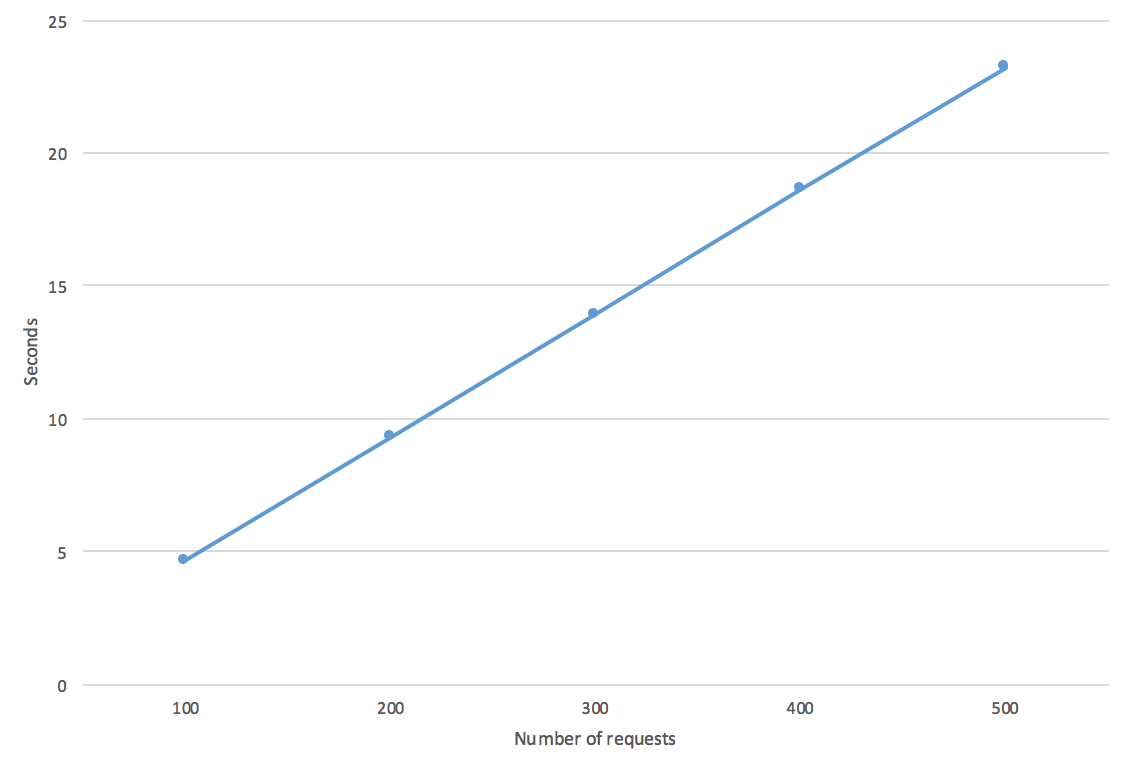
\includegraphics[width=\linewidth]{sequential_numrequests_seconds.png}
    \caption{Linear growth of processing time as number of requests increases.}
    \label{fig:seq_numrequests_seconds}
  \end{center}
\end{figure}

The 40 ms artificial delay we introduced when processing the requests has a significant effect on the performance. If the delay is removed we can serve 100 requests in approximately 0,11 seconds, compared to the 4,66 seconds it took us with the delay in place.

Interestingly, running the test with concurrent requests gives different results than if the requests are only sent out sequentially. Processing of 100 requests (N=100), sent using 100 concurrent request processes (C=100) took 4,09 seconds, compared to the 4,66 seconds it took for sequential requests. This is likely because we save ourselves the time it takes to prepare and send out the requests sequentially on the client; after one request has been sent the client requires some time before it can send out the next one. Using concurrent requests is a good simulation for what would happen if the benchmark were run on several machines at the same time.

\section{Concurrent Rudy}

To improve the performance of the server the best approach is to modify it to handle incoming requests concurrently. This way an incoming request from a client could be served immediately instead of waiting its turn.
To achieve this the server uses a pool of processes to handle incoming requests. The pool is configured with a limit on how many handler processes can be active at the same time. If a handler process is available in the pool when a request arrives it is handled immediately, otherwise it is put on hold until a handler process becomes available. By using a process pool instead of just creating a new process for each incoming request we are able to limit the number of processes that are active at any given time, thereby preserving computational resources.

The implementation consists of two main parts; a \texttt{PoolManager} process and a \texttt{Pool} process. When a request comes in, the server process sends a message to the \texttt{PoolManager} process asking it to handle the request. The \texttt{PoolManager} process then sends a message to the \texttt{Pool} process asking it to spawn a handler process for the request. If there is a handler available in the pool the \texttt{Pool} process will spawn the handler process and decrease the number of available handlers in the pool. If the pool is empty however, the \texttt{Pool} process will send a message back to the \texttt{PoolManager} process notifying it that the request was rejected. The \texttt{PoolManager} process then keeps all rejected requests in a queue in order to be able to serve them later when a handler becomes available. When a handler process finishes, it sends a message to the \texttt{Pool} process to notify it. The \texttt{Pool} process then increases the number of available handlers in the pool and sends a message to the \texttt{PoolManager} process notifying it that a handler just became available. The \texttt{PoolManager} process will then request a handler process again for the request at the front of the queue of previously rejected requests.

\subsection{Evaluation}

The concurrent version of the server offers significant performance improvements over the sequential server. Again, all tests were done with a 40 ms artificial processing delay for the requests and all test results are the average of 10 runs for each test case.

The best test case (100 concurrent requests, with a process pool of size 100) shows that we are now able to serve approximately 785 requests per second. The test results for different pool sizes are shown in table \ref{tab:concurrent_results}.

\begin{table}[h]
\centering
\begin{tabular}{lcc}
Parameters & Time (sec)\\\hline
C=100, N=100, PS=1 & 4,033926751\\\hline
C=100, N=100, PS=10 & 0,380211564\\\hline
C=100, N=100, PS=20 & 0,269060245\\\hline
C=100, N=100, PS=30 & 0,214021727\\\hline
C=100, N=100, PS=40 & 0,196885518\\\hline
C=100, N=100, PS=50 & 0,150800505\\\hline
C=100, N=100, PS=60 & 0,152701674\\\hline
C=100, N=100, PS=70 & 0,155557886\\\hline
C=100, N=100, PS=80 & 0,143427895\\\hline
C=100, N=100, PS=90 & 0,138553424\\\hline
C=100, N=100, PS=100 & 0,127274186\\\hline
\end{tabular}
\caption{Concurrent server test results. C: Number of concurrent requests, N: Number of requests, PS: Pool size}
\label{tab:concurrent_results}
\end{table}

The time it takes to serve these 100 requests is however not linearly decreasing with increasing pool size, according to the test results. This is apparent in figure \ref{fig:concurrent_poolsize_seconds}. This may be due to outliers in the test result data, as well as other factors. Some test runs received errors for some of their requests, giving unexpected test results. This was not investigated further. However, the trend is towards lower processing time as the pool size increases.

\begin{figure}[h]
  \begin{center}
    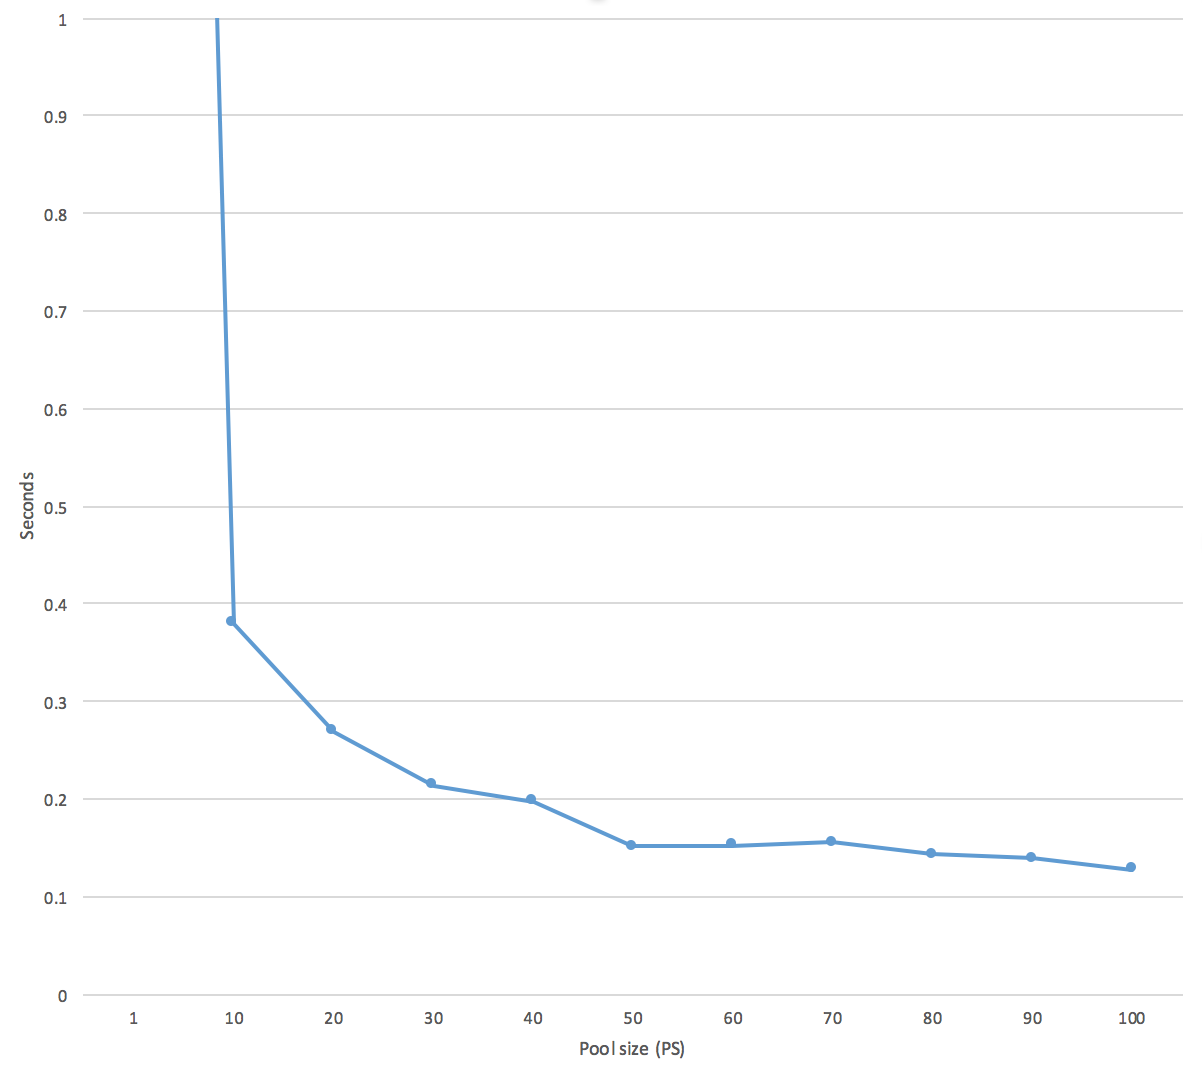
\includegraphics[width=\linewidth]{concurrent_poolsize_seconds.png}
    \caption{Performance increase with increasing pool size. Note: Data point for PS=1 not visible.}
    \label{fig:concurrent_poolsize_seconds}
  \end{center}
\end{figure}

All of the tests previously discussed were made using 100 concurrent requests (C=100). Having all of the requests sent in parallel (C==N) best simulates real world load on the server, as if multiple machines were accessing it at the same time.

\section{Conclusions}

It is obvious that the benefits of having a multithreaded web server are significant. The concurrent version of the server is able to handle 785 requests per second while the sequential server can only handle 21 requests per second.

\end{document}
